\documentclass{report}
\usepackage[spanish]{babel}
\usepackage[utf8]{inputenc}
\usepackage{graphicx, longtable, float, titlesec, hyperref}

\hypersetup{
    hidelinks = true
}

\titleformat{\chapter}[display]
  {\normalfont\bfseries}{}{0pt}{\Huge}

\begin{document}
    \begin{titlepage}
        \centering
        
\includegraphics[width=0.6\textwidth]{./img/miscelanio/logo.jpg}\\
        \vspace{1cm}
        \LARGE Sistemas de Gestión de Seguridad de Sistemas de Información\\
        \vspace{0.5cm}
        \Large Ingeniería Informática de Gestión y Sistemas de Información\\
        \vspace{3cm}
        \Huge Sistema Web\\
        \vspace{2.5cm}
        \Large Autores:\\
        \vspace{0.2cm}
        \large Xabier Gabiña\\
        \large Ainhize Martinez\\
        \large Marcos Martín\\
        \vfill
        \today
    \end{titlepage}
    \tableofcontents
    \chapter{Introduccion}
        La finalidad de esta etapa del proyecto consiste en garantizar la seguridad y robustez de la página web desarrollada en la fase inicial del proyecto. Con el propósito de lograr este objetivo, se recurrirá a la aplicación de diversas herramientas y técnicas que han sido abordadas y exploradas a lo largo del curso. El enfoque principal de esta fase se centra en identificar y abordar posibles vulnerabilidades y debilidades de seguridad en el sistema, a fin de implementar medidas correctivas y fortalecer la integridad de la plataforma web.
        
        Este proceso implica la utilización de herramientas especializadas, como ZAP, SQLMap, Nmap y Metasploit, que permiten evaluar y poner a prueba la infraestructura de seguridad de la página web. A través de su empleo, se llevará a cabo un exhaustivo análisis que permitirá descubrir posibles fallos o vulnerabilidades que puedan ser aprovechadas por actores maliciosos, poniendo en riesgo la integridad de los datos y la privacidad de los usuarios.
        
        El objetivo último es la identificación, documentación y solución de posibles vulnerabilidades, lo que contribuirá a elevar la seguridad y confiabilidad de la página web. A medida que se avance en este proceso, se aplicarán estrategias y medidas correctivas para abordar los hallazgos identificados y se establecerán salvaguardias que minimicen el riesgo de futuros incidentes de seguridad.
        
        Este proyecto representa un ejercicio académico valioso que no solo demuestra la comprensión de los conceptos de seguridad informática, sino que también ofrece la oportunidad de aplicar de manera práctica las habilidades adquiridas en la detección y mitigación de riesgos en entornos web. A través de esta experiencia, se espera adquirir un conocimiento más profundo y aplicable en el campo de la seguridad informática y estén mejor preparados para enfrentar desafíos en el mundo real.
    \chapter{Primera auditoria}
        La idea de esta auditoria es la de encontrar los fallos de seguridad que tiene nuestro sistema web para en el posterior capitulo de este documento comentarlos y solucionarlos.\\
        \section{ZAP}
            Para empezar con la primera auditoria ejecutaremos el proxy ZAP como se nos ha propuesto en clase.
            Al ejecutarla en nuestra pagina web nos encontramos con el siguiente listado de errores:
            \begin{figure}[H]
                \centering
                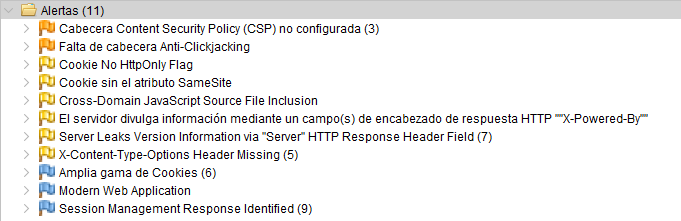
\includegraphics[width=\textwidth]{./img/audit1/zap1.png}
                \caption{Listado de errores de la primera auditoria}
            \end{figure}
            Como podemos ver en la imagen, tenemos un total de 11 errores, los cuales iremos comentando uno a uno en los siguientes apartados y solucionando.
        \clearpage
        \section{sqlmap}
        \clearpage
        \section{nmap}
        \clearpage
        \section{Metaexploit}
        \clearpage
    \chapter{Vulnerabilidades}
        \section{Rotura de control de acceso}
            La rotura de control de acceso es una vulnerabilidad que permite a un atacante acceder a recursos restringidos o privilegiados, ya sea por un error en la implementación de la autenticación y autorización o por un error en la lógica de control de acceso.
            \subsection{Control de acceso}
                \subsubsection{Descripción}
                    En nuestro sistema, un usuario puede modificar sus datos personales, pero también puede modificar los datos de otros usuarios. 
                    Esto es un fallo de rotura de control de acceso ya que un usuario no debería poder modificar los datos de otro usuario.
                \subsubsection{PoC}
                    Pongamos en el ejemplo que tenemos dos usuarios, Admin y Xabier con sus repectivas IDs
                    \begin{figure}[H]
                        \centering
                        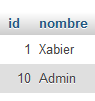
\includegraphics[width=0.2\textwidth]{./img/vulnerabilidades/3.1/1.1.png}
                        \caption{Datos de Usuarios}
                    \end{figure}
                    Si desde inspeccionar elementos hacemos click sobre el boton 'Perfil' este nos mostrara el link el cual se ve asi:
                    \begin{figure}[H]
                        \centering
                        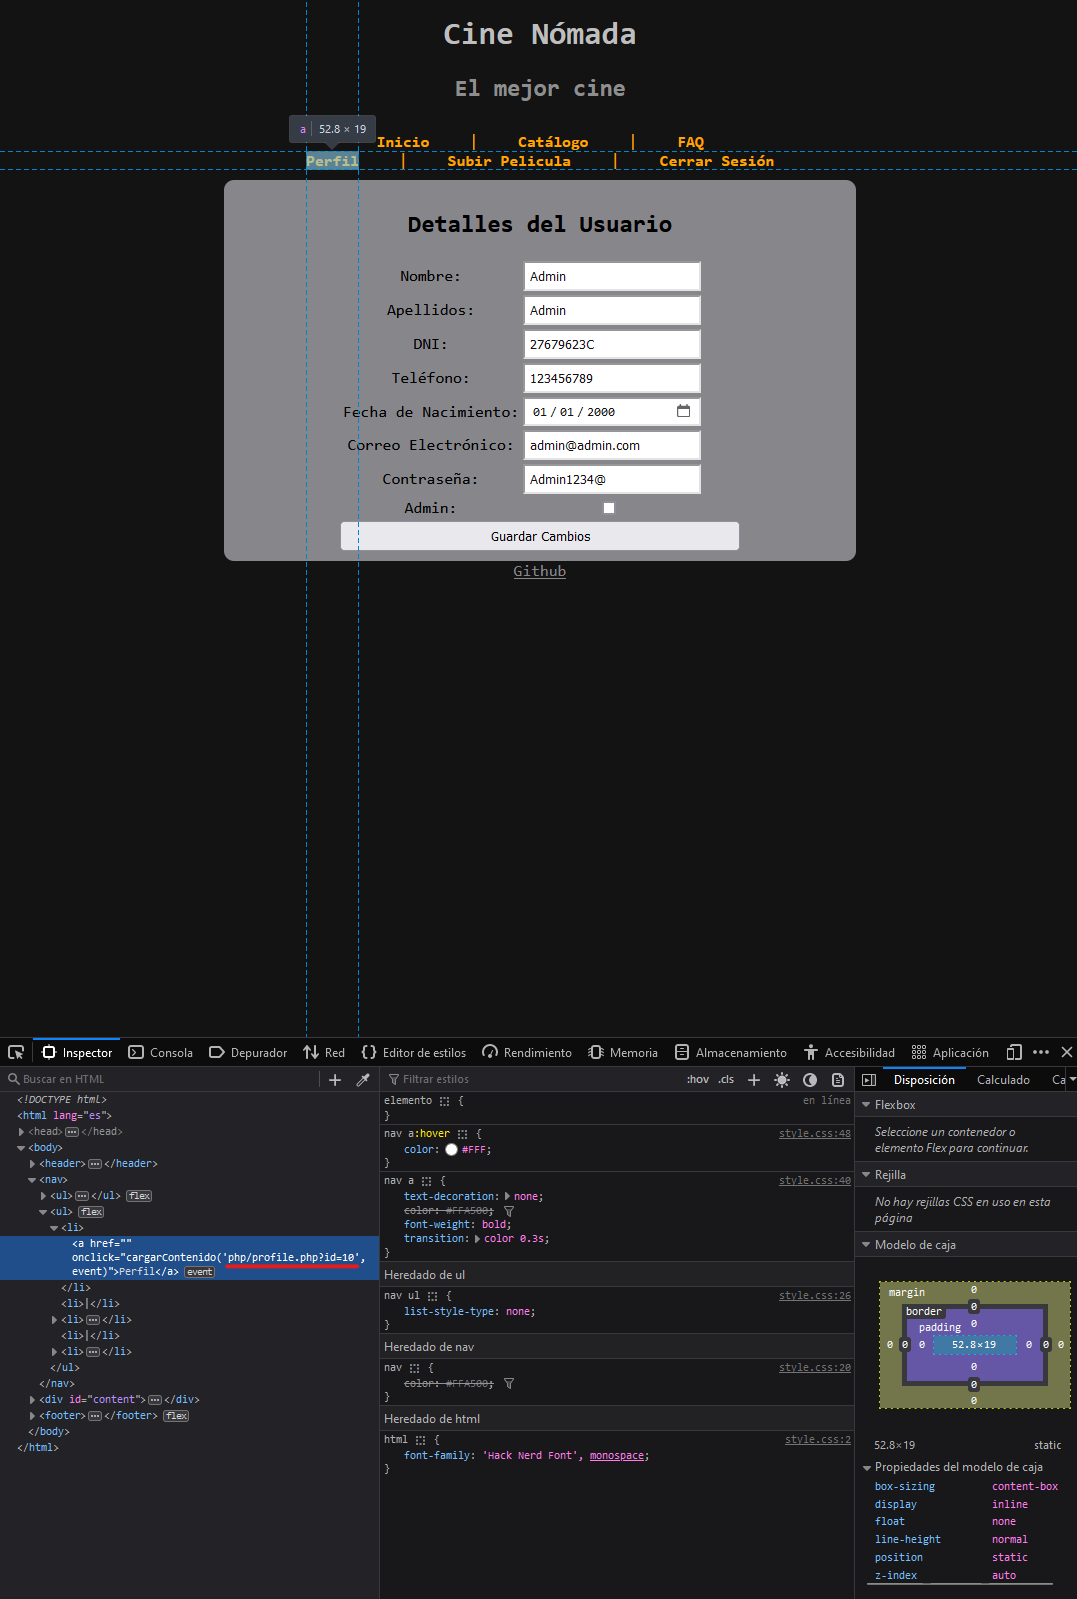
\includegraphics[width=0.8\textwidth]{./img/vulnerabilidades/3.1/1.2.png}
                        \caption{Perfil de Admin}
                    \end{figure}
                    Si alteramos el valor de ?id=X por en este caso la id de Xabier (La ID 1) podemos acceder a sus datos
                    \begin{figure}[H]
                        \centering
                        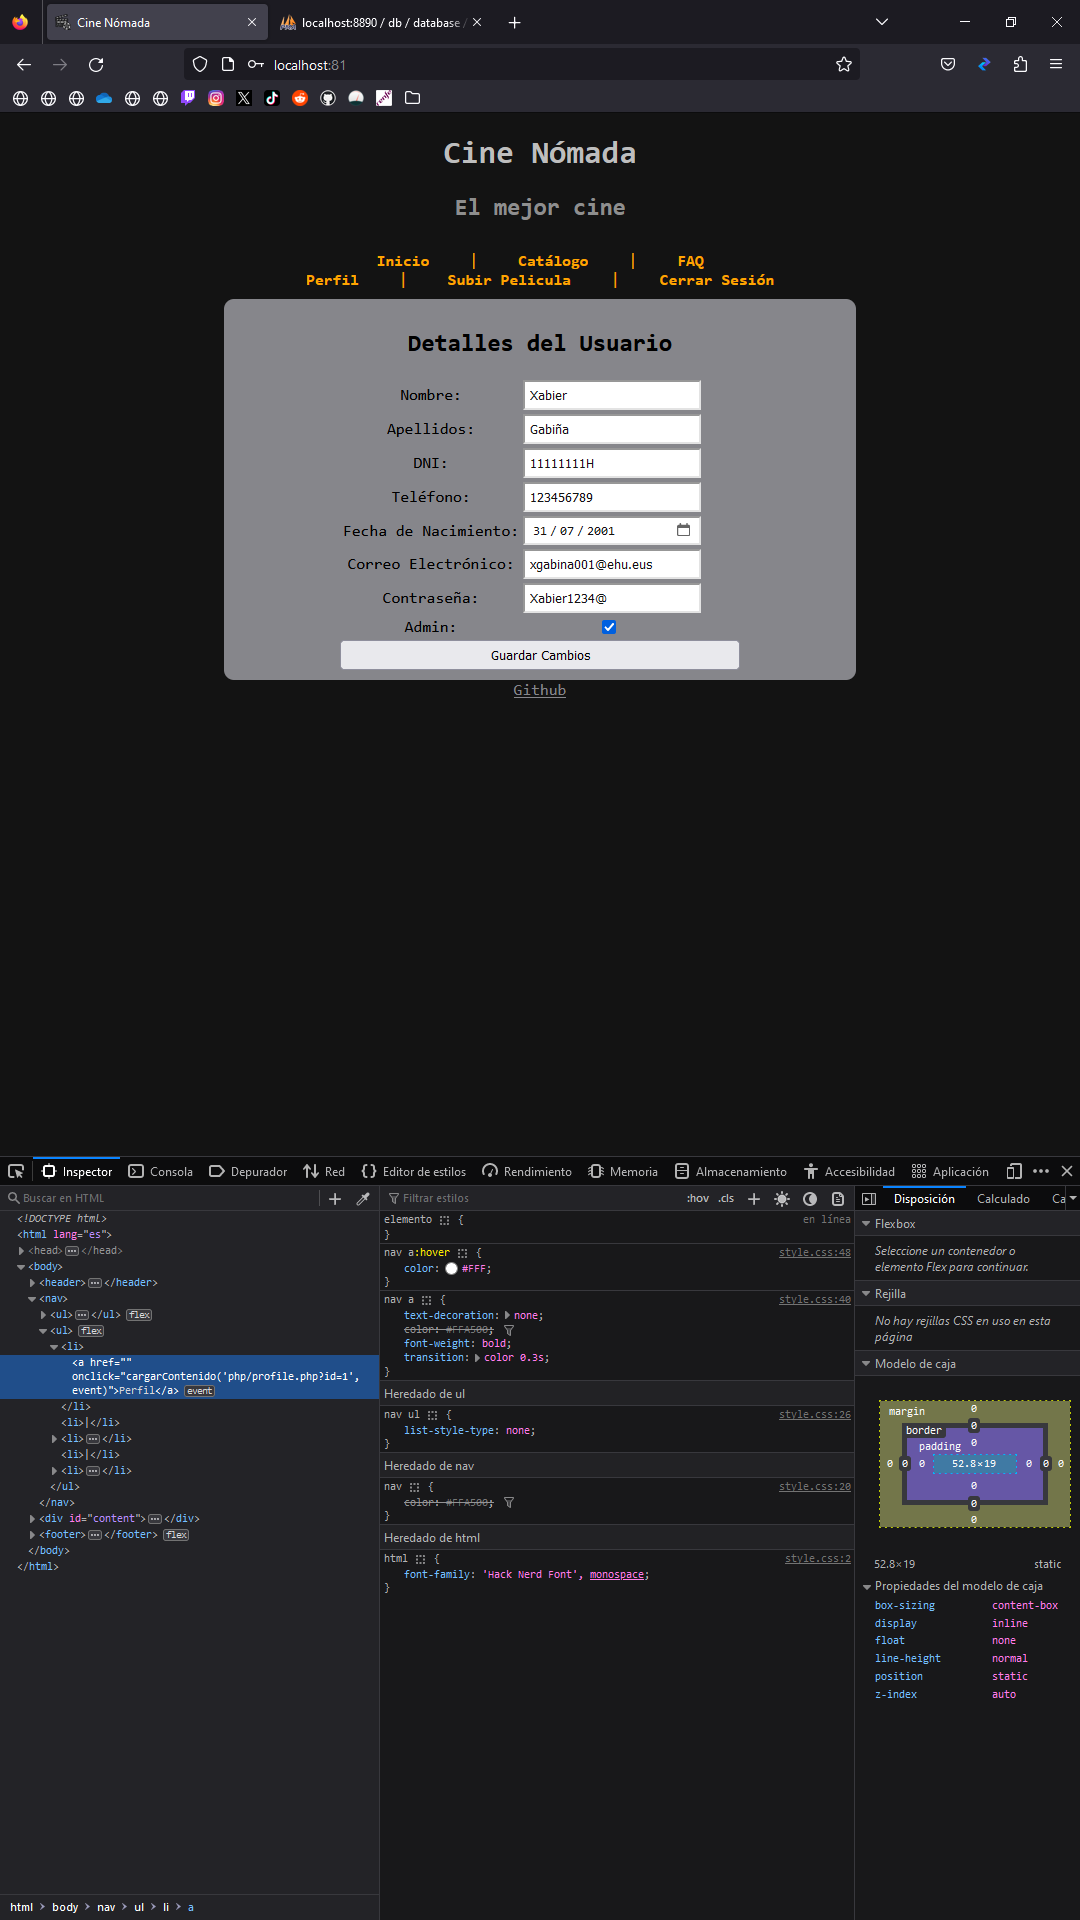
\includegraphics[width=\textwidth]{./img/vulnerabilidades/3.1/1.3.png}
                        \caption{Perfil de Xabier}
                    \end{figure}
                \subsubsection{Solución}
                    Para solucionar este problema, hemos añadido una comprobación en el código que comprueba que el usuario que está intentando modificar los datos es el mismo que el usuario que está logueado en el sistema.
                    \begin{figure}[H]
                        \centering
                        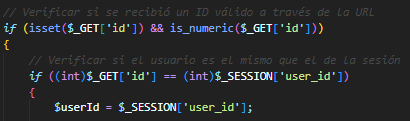
\includegraphics[width=\textwidth]{./img/vulnerabilidades/3.1/1.4.png}
                        \caption{Comprobación de usuario}
                    \end{figure}
                    Esta misma error tambien ha sido corregido en el catalogo.
            \clearpage       
        \section{Fallos criptográficos}
            Los "fallos criptográficos" se refieren a debilidades o errores en el diseño, implementación o uso de algoritmos criptográficos que comprometen la seguridad de la información protegida mediante técnicas de cifrado y protección.
            \subsection{Cifrado de extremo a extremo}
                \subsubsection{Descripción}
                El cifrado de extremo a extremo es un método de seguridad informática en el que la información se cifra en el punto de origen y solo se descifra en el punto de destino. Esto significa que los datos están protegidos durante su transmisión y solo son legibles para la parte destinataria que posee la clave de descifrado correspondiente.
                \subsubsection{Solución}
                    Para solucionar este problema configuraremos nuestro servidor para que cifre y rediriga todo el trafico a HTTPS.
                    
                    Creamos un certificado SSL autofirmado dentro del Dockerfile.
                    
                    Creamos una regla para redirigir el trafico entrante del puerto 80 al puerto 443.
                    \begin{figure}[H]
                        \centering
                        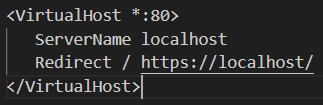
\includegraphics[width=\textwidth]{./img/vulnerabilidades/3.2/1.1.png}
                        \caption{Redireccion de trafico}
                    \end{figure}
                    
                    Tambien debemos decir al puerto 443 que use el certificado SSL que hemos creado.
                    \begin{figure}[H]
                        \centering
                        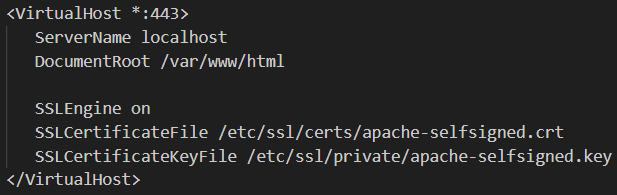
\includegraphics[width=\textwidth]{./img/vulnerabilidades/3.2/1.2.png}
                        \caption{Certificado SSL}
                    \end{figure}
            \clearpage
            \subsection{Almacenamiento de contraseñas}
                \subsubsection{Descripción}
                    En nuestro sistema, no se almacenan las contraseñas de los usuarios de forma segura, lo que permite que un atacante pueda obtener las contraseñas de los usuarios.
                \subsubsection{PoC}
                    Si un atacante consigue acceso a la base de datos, puede obtener las contraseñas de los usuarios en texto plano.
                    \begin{figure}[H]
                        \centering
                        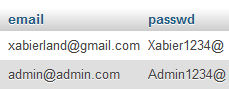
\includegraphics[width=\textwidth]{./img/vulnerabilidades/3.2/2.1.png}
                        \caption{Contraseñas en texto plano}
                    \end{figure}
                \subsubsection{Solución}
                    Para solucionar este problema de la mejor forma posible debemos tener tres puntos bien definidos:
                    \begin{enumerate}
                        \item Cofigurar el factor de costo apropiado
                        \begin{itemize}
                            \item El factor de costo (work factor) en bcrypt determina el número de iteraciones utilizadas en el cálculo del hash. Un valor mayor implica una contraseña más segura, pero también requiere más tiempo para calcular el hash. Un valor razonable es 12 o más, dependiendo del hardware y las necesidades de rendimiento.
                        \end{itemize}
                        \item Usar un algoritmo de cifrado seguro.
                        \begin{itemize}
                            \item En nuestro caso usaremos BCrypt. CRYPT\_BLOWFISH se usa para crear el hash. Producirá un hash estándar compatible con crypt() utilizando el identificador \texttt{"\$2y\$"}. El resultado siempre será un string de 60 caracteres, o false en caso de error.
                        \end{itemize}
                        \item Generar un semilla aleatoria para cada usuario.
                        \begin{itemize}
                            \item BCrypt ya gestiona las semillas de forma automatica y en el manual de PHP no recomiendan su uso de otra manera. Mas informacion en \url{https://www.php.net/manual/es/function.password-hash.php}
                        \end{itemize}
                    \end{enumerate}
                    \begin{figure}[H]
                        \centering
                        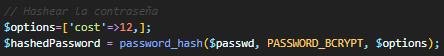
\includegraphics[width=\textwidth]{./img/vulnerabilidades/3.2/2.2.png}
                        \caption{Contraseñas encriptadas}
                    \end{figure}
            \clearpage
            \subsection{Configuracion erronea de las Cookies}
                \subsubsection{Descripción}
                    La configuración errónea de las cookies se refiere a la práctica de establecer parámetros o atributos de las cookies de manera inadecuada, lo que puede tener consecuencias negativas en términos de seguridad, privacidad y funcionalidad en una aplicación web.                
                \subsubsection{Solución}
                    Para solucionar este problema, hemos añadido una configuración segura a las cookies de nuestro sitio web.
                    \begin{figure}[H]
                        \centering
                        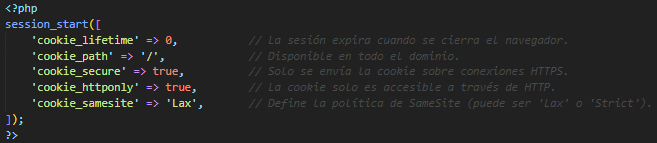
\includegraphics[width=\textwidth]{./img/vulnerabilidades/3.2/3.1.png}
                        \caption{Configuración de las cookies}
                    \end{figure}
            \clearpage
        \section{Inyección}
            En el ámbito de la seguridad informática y el desarrollo de software, el término "inyección" se refiere a una clase de vulnerabilidades que permite a un atacante introducir y ejecutar código malicioso en una aplicación o sistema. 
            \subsection{SQL Injection}
                \subsubsection{Descripción}
                    La inyección SQL es una vulnerabilidad de seguridad informática que permite a un atacante modificar las consultas SQL que se ejecutan en una base de datos subyacente. Esto puede permitir a un atacante obtener información confidencial, alterar o eliminar datos, o incluso comprometer completamente el sistema.
                \subsubsection{PoC}
                \subsubsection{Solución}
                    Para solucionar este problema, hemos modificado el codigo que procesa las consultas SQL para que no se puedan inyectar consultas SQL.
                    \begin{figure}[H]
                        \centering
                        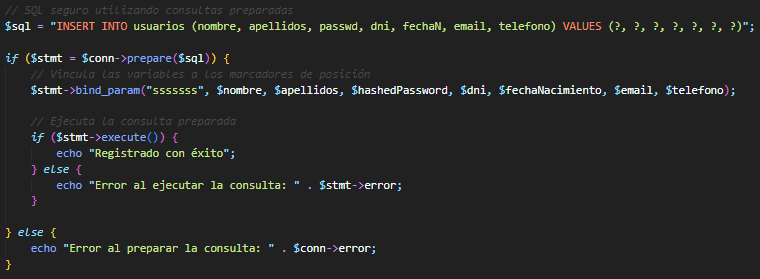
\includegraphics[width=\textwidth]{./img/vulnerabilidades/3.3/1.1.png}
                        \caption{Parametrizar consulta SQL}
                    \end{figure}
            \clearpage
            \subsection{Cross-Site Scripting (XSS)}
                \subsubsection{Descripción}
                    El Cross-Site Scripting (XSS) es una vulnerabilidad de seguridad informática que permite a un atacante inyectar código malicioso (por lo general JavaScript) en páginas web que son vistas por otros usuarios. El XSS permite a los atacantes ejecutar scripts en el navegador de un usuario, lo que puede secuestrar sesiones de usuario, desfigurar sitios web, robar información confidencial y distribuir malware.
                \subsubsection{Solución}
                    La solucion a este problema se vera mas adelante en la seccion 3.5.5
            \clearpage
            \subsection{Cross-Site Request Forgery}
                \subsubsection{Descripción}
                    El Cross-Site Request Forgery (CSRF) es una vulnerabilidad de seguridad informática que permite a un atacante forzar a un usuario autenticado a ejecutar acciones no deseadas en una aplicación web en la que confía. El CSRF puede utilizarse para realizar acciones como transferencias de fondos, cambios de contraseñas, compras, etc.
                \subsubsection{Solución}
                    Para solucionar este problema, hemos añadido un token CSRF a nuestro sitio web.
                    \begin{figure}[H]
                        \centering
                        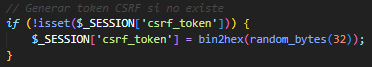
\includegraphics[width=\textwidth]{./img/vulnerabilidades/3.3/3.1.png}
                        \caption{Token CSRF}
                    \end{figure}
                    \begin{figure}[H]
                        \centering
                        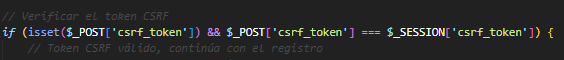
\includegraphics[width=\textwidth]{./img/vulnerabilidades/3.3/3.2.png}
                        \caption{Comprobacion de token CSRF}
                    \end{figure}
            \clearpage
        \section{Diseño inseguro}
            El "diseño inseguro" se refiere a la presencia de debilidades fundamentales en el diseño de una aplicación web que pueden ser explotadas por atacantes para comprometer la seguridad.
            \subsection{Reutilizacion de codigos seguros}
                \subsubsection{Descripción}
                    La reutilización de código seguro se refiere a la práctica de aprovechar componentes de software previamente probados y seguros en lugar de escribir código desde cero. Esto no solo puede acelerar el desarrollo de software, sino que también puede reducir el riesgo de introducir vulnerabilidades de seguridad.
                \subsubsection{Solución}
                    En nuestro proyecto se han implementado estas practicas mediante la reutilización del archivo validar.js en el que se encuentran las funciones de validación de todos los formularios de nuestro sitio web.
                    \begin{figure}[H]
                        \centering
                        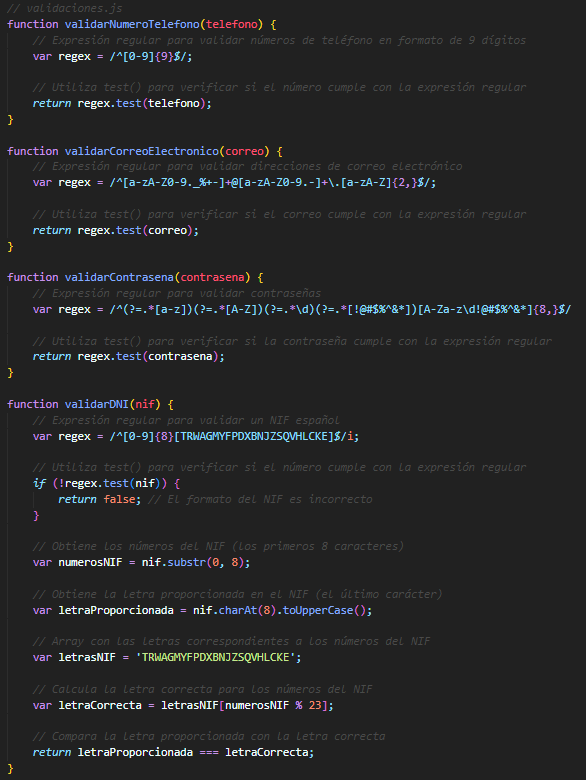
\includegraphics[width=\textwidth]{./img/vulnerabilidades/3.4/1.1.png}
                        \caption{Validacion de formularios}
                    \end{figure}
            \clearpage
        \section{Configuración de seguridad insuficiente}
            La configuración de seguridad incorrecta o insuficiente se refiere a ajustes o parámetros de seguridad que no están adecuadamente configurados para proteger un sistema, aplicación, red o servicio. Puede haber varias áreas en las que la configuración de seguridad puede ser insuficiente o incorrecta, lo que podría dejar un sistema vulnerable a amenazas y ataques.
            \subsection{Despliegue seguro}
                \subsubsection{Descripción}
                    Es importante que a la hora de montar nuestro servidor web no haya archivos que puedan ser accesibles desde el exterior y que puedan contener informacion sensible como contraseñas. Esto a nosotros nos ocurre en el docker-compose.yml
                \subsubsection{Solución}
                    Hemos creado un .env donde se almacenan las contraseñas y demas informacion sensible y hemos añadido el archivo al .gitignore para que no se suba al repositorio.
                    Dado que esto es un trabajo el .env sera incluido para poder comprobar que funciona correctamente.
                    \begin{figure}[H]
                        \centering
                        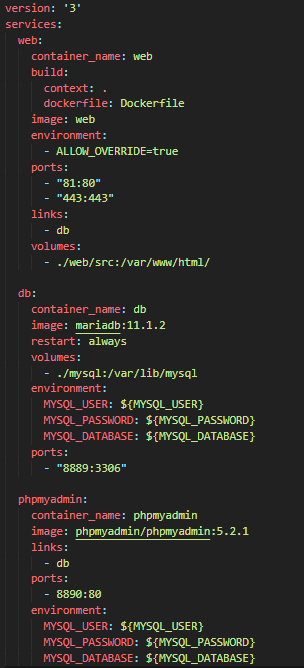
\includegraphics[width=\textwidth]{./img/vulnerabilidades/3.5/1.1.png}
                        \caption{docker-compose sin informacion sensible}
                    \end{figure}
            \clearpage
            \subsection{Cabecera CSP}
                \subsubsection{Descripción}
                    Las cabeceras CSP son una medida de seguridad utilizada en la programación web para mitigar los riesgos asociados con ataques de Cross-Site Scripting (XSS) y otros tipos de ataques de inyección de código malicioso en páginas web.
                \subsubsection{Solución}
                    Para solucionar este problema, hemos añadido una cabecera 'Content-Security-Policy' con los siguientes valores:
                    \begin{figure}[H]
                        \centering
                        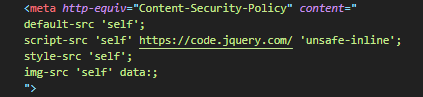
\includegraphics[width=\textwidth]{./img/vulnerabilidades/3.5/2.1.png}
                        \caption{Cabecera CSP}
                    \end{figure}
            \clearpage
            \subsection{Cabecera Cache-Control}
                \subsubsection{Descripción}
                    Las cabeceras 'Cache-Control' son utilizadas en las respuestas HTTP enviadas por un servidor web para controlar cómo los recursos web deben ser almacenados en la memoria caché del navegador o en servidores intermedios (como proxies) y cómo se deben comportar en términos de almacenamiento y actualización. Estas cabeceras son fundamentales para gestionar la eficiencia de la carga de páginas web, la seguridad y la privacidad.
                \subsubsection{Solución}
                    Para solucionar este problema crearemos una cabecera 'Cache-Control' con el valor 'no-store' para que el navegador no almacene en cache la pagina.
                    \begin{figure}[H]
                        \centering
                        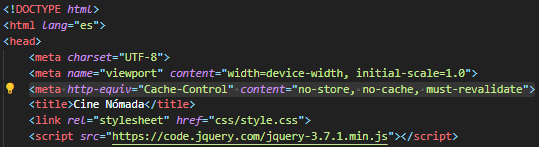
\includegraphics[width=\textwidth]{./img/vulnerabilidades/3.5/3.1.png}
                        \caption{Cabecera Cache-Control}
                    \end{figure}
            \clearpage
            \subsection{Cabecera HSTS}
                \subsubsection{Descripción}
                    Las cabeceras HSTS (HTTP Strict Transport Security) son una medida de seguridad utilizada en la programación web para garantizar que las comunicaciones entre un navegador web y un sitio web se realicen a través de una conexión segura y encriptada utilizando el protocolo HTTPS (HTTP Secure). HSTS ayuda a prevenir ataques de tipo man-in-the-middle (MitM) que podrían exponer datos sensibles o comprometer la seguridad de la comunicación.
                \subsubsection{Solución}
                    Para solucionar este problema, hemos añadido una cabecera 'Strict-Transport-Security' con los siguientes valores:
                    \begin{figure}[H]
                        \centering
                        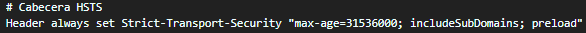
\includegraphics[width=\textwidth]{./img/vulnerabilidades/3.5/4.1.png}
                        \caption{Cabecera HSTS}
                    \end{figure}
            \clearpage
            \subsection{Cabecera X-XSS-Protection}
                \subsubsection{Descripción}
                Las cabeceras "X-XSS-Protection" son una medida de seguridad utilizada en la programación web para ayudar a prevenir ataques de tipo Cross-Site Scripting (XSS). Los ataques XSS ocurren cuando un atacante inyecta código JavaScript malicioso en una página web, que luego se ejecuta en el navegador de un usuario sin su conocimiento. Estas cabeceras se utilizan para controlar y mitigar estos ataques.
                \subsubsection{Solución}
                    Para solucionar este problema, hemos añadido una cabecera 'X-XSS-Protection' con los siguientes valores:
                    \begin{figure}[H]
                        \centering
                        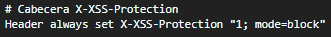
\includegraphics[width=\textwidth]{./img/vulnerabilidades/3.5/5.1.png}
                        \caption{Cabecera X-XSS-Protection}
                    \end{figure}
            \clearpage
            \subsection{Cabecera X-Content-Type-Options}
                \subsubsection{Descripción}
                Las cabeceras "X-Content-Type-Options" son una medida de seguridad utilizada en la programación web para mitigar ciertos tipos de ataques, como ataques de tipo MIME-sniffing. Estas cabeceras se utilizan para controlar cómo el navegador web interpreta y muestra el contenido de una página web.
                \subsubsection{Solución}
                    Para solucionar este problema, hemos añadido una cabecera 'X-Content-Type-Options' con los siguientes valores:
                    \begin{figure}[H]
                        \centering
                        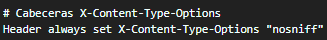
\includegraphics[width=\textwidth]{./img/vulnerabilidades/3.5/6.1.png}
                        \caption{Cabecera X-Content-Type-Options}
                    \end{figure}
            \clearpage
            \subsection{Cabecera X-Frame-Options}
                \subsubsection{Descripción}
                    Las cabeceras "X-Frame-Options" son una medida de seguridad utilizada en la programación web para controlar si una página web puede ser incrustada o mostrada dentro de un marco (frame) de otro sitio web. Estas cabeceras se utilizan para prevenir ataques de clickjacking, en los cuales un atacante puede ocultar contenido malicioso detrás de una página legítima y engañar a los usuarios para que hagan clic en elementos sin su consentimiento.
                \subsubsection{Solución}
                    Para solucionar este problema, hemos añadido una cabecera 'X-Frame-Options' con los siguientes valores:
                    \begin{figure}[H]
                        \centering
                        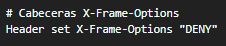
\includegraphics[width=\textwidth]{./img/vulnerabilidades/3.5/7.1.png}
                        \caption{Cabecera X-Frame-Options}
                    \end{figure}
            \clearpage
            \subsection{Cabecera X-Permitted-Cross-Domain-Policies}
                \subsubsection{Descripción}
                    La cabecera X-Permitted-Cross-Domain-Policies permite a los propietarios del contenido controlar cómo los documentos son tratados en contextos de navegación cruzada.
                \subsubsection{Solución}
                    Para solucionar este problema crearemos una cabecera 'X-Permitted-Cross-Domain-Policies' con el valor 'none' para que el navegador no permita que se usen caracteristicas y APIs en los contenidos de una pagina.
                    \begin{figure}[H]
                        \centering
                        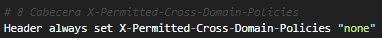
\includegraphics[width=\textwidth]{./img/vulnerabilidades/3.5/8.1.png}
                        \caption{Cabecera X-Permitted-Cross-Domain-Policies}
                    \end{figure}
            \clearpage
            \subsection{Cabecera X-DNS-Prefetch-Control}
                \subsubsection{Descripción}
                    La cabecera X-DNS-Prefetch-Control es una cabecera HTTP que se utiliza para controlar la funcionalidad de prefetching DNS en los navegadores. El prefetching DNS es una técnica que los navegadores utilizan para anticiparse a las solicitudes DNS antes de que un usuario haga clic en un enlace. Esto puede acelerar la carga de páginas al preresolver los nombres de dominio antes de que se soliciten explícitamente.
                    Esto puede provocar que el navegador realice peticiones a dominios que no son de confianza, dar informacion de dominios sensibles, etc.
                \subsubsection{Solución}
                    Para solucionar este problema crearemos una cabecera 'X-DNS-Prefetch-Control' con el valor 'off' para que el navegador no permita que se precarge contenido de la pagina.
                    \begin{figure}[H]
                        \centering
                        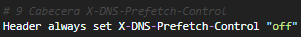
\includegraphics[width=\textwidth]{./img/vulnerabilidades/3.5/9.1.png}
                        \caption{Cabecera X-DNS-Prefetch-Control}
                    \end{figure}
            \clearpage
            \subsection{Cabecera X-Download-Options}
                \subsubsection{Descripción}
                    La cabecera X-Download-Options es una cabecera HTTP que se utiliza para controlar cómo ciertos navegadores manejan la descarga de archivos. Esta cabecera tiene un propósito específico en el contexto de Internet Explorer (IE) y se utiliza para mitigar el riesgo de ejecución automática de archivos descargados que podrían ser maliciosos.
                \subsubsection{Solución}
                    Para solucionar este problema crearemos una cabecera 'X-Download-Options' con el valor 'noopen' para que el navegador no permita que se ejecuten los archivos descargados.
                    \begin{figure}[H]
                        \centering
                        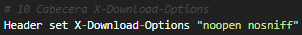
\includegraphics[width=\textwidth]{./img/vulnerabilidades/3.5/10.1.png}
                        \caption{Cabecera X-Download-Options}
                    \end{figure}
            \clearpage
            \subsection{Cabecera Referrer-Policy}
                \subsubsection{Descripción}
                    Esta cabecera controla cómo se incluye el encabezado Referer en las solicitudes. Puedes configurarlo para reducir la cantidad de información sensible enviada en las solicitudes de referencia.
                \subsubsection{Solución}
                    Para solucionar este problema crearemos una cabecera 'Referrer-Policy' con el valor 'no-referrer' para que el navegador no envie informacion sensible en las solicitudes de referencia.
                    \begin{figure}[H]
                        \centering
                        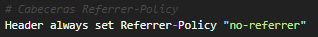
\includegraphics[width=\textwidth]{./img/vulnerabilidades/3.5/11.1.png}
                        \caption{Cabecera Referrer-Policy}
                    \end{figure}
            \clearpage
            \subsection{Cabecera Feature-Policy}
                \subsubsection{Descripción}
                    La cabecera 'Feature-Policy' permite que un sitio controle qué características y APIs pueden ser utilizadas por los contenidos de una página.
                \subsubsection{Solución}
                    Para solucionar este problema crearemos una cabecera 'Feature-Policy' con el valor 'none' para que el navegador no permita que se usen caracteristicas y APIs en los contenidos de una pagina.
                    \begin{figure}[H]
                        \centering
                        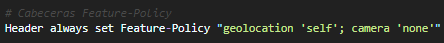
\includegraphics[width=\textwidth]{./img/vulnerabilidades/3.5/12.1.png}
                        \caption{Cabecera Feature-Policy}
                    \end{figure}
            \clearpage
            \subsection{Cabecera Expect-CT}
                \subsubsection{Descripción}
                    Las cabeceras 'Expect-CT' ayuda a proteger al usuario contra ataques de certificate transparency.
                \subsubsection{Solución}
                    Para solucionar este problema crearemos una cabecera 'Expect-CT' con el valor 'max-age=86400' para que el navegador no permita que se usen caracteristicas y APIs en los contenidos de una pagina.
                    \begin{figure}[H]
                        \centering
                        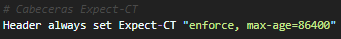
\includegraphics[width=\textwidth]{./img/vulnerabilidades/3.5/13.1.png}
                        \caption{Cabecera Expect-CT}
                    \end{figure}
            \clearpage
            \subsection{Configuracion PHP}
                \subsubsection{Descripción}
                    Cuando usamos PHP en un servidor web es importante el configurarlo de forma segura para evitar que se filtre informacion que pueda ayudar a los atacantes a encontrar una vulnerabilidad en nuestro sistema.
                \subsubsection{Solución}
                    Hemos ocultado la version de PHP en las peticiones a nuestro servidor para evitar que un atacante pueda usar esta informacion para encontrar una vulnerabilidad en nuestro sistema. Para ello hemos creado el php.ini
                    \begin{figure}[H]
                        \centering
                        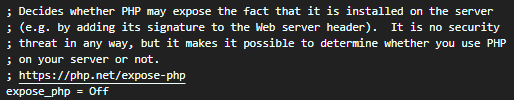
\includegraphics[width=\textwidth]{./img/vulnerabilidades/3.5/14.1.png}
                        \caption{Ocultar version de PHP}
                    \end{figure}
            \clearpage
            \subsection{Configuracion Apache}
                \subsubsection{Descripción}
                    Al igual que con PHP en el punto anterior es importante configurar Apache para que muestre la minima informacion al exterior.
                \subsubsection{Solución}
                    Para ello, al igual que con PHP, hemos ocultado las versiones del servidor para evitar en la medida de lo posible que el atacante encuntre vulnerabilidad en nuestro servidor. Para ello hemos editado el apache2.conf
                    \begin{figure}[H]
                        \centering
                        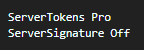
\includegraphics[width=\textwidth]{./img/vulnerabilidades/3.5/15.1.png}
                        \caption{Ocultar version de Apache}
                    \end{figure}
            \clearpage
        \section{Componentes vulnerables y obsoletos}
            Se refiere a partes o elementos dentro de un sistema, software o hardware, que presentan vulnerabilidades de seguridad debido a su antigüedad o a la falta de actualizaciones.
            \subsection{Control de versiones de los componentes}
                \subsubsection{Descripción}
                    Es crítico mantener actualizados los sistemas operativos y el software de seguridad con las últimas actualizaciones y parches de seguridad.
                \subsubsection{Solución}
                    Para solucionar este problema, hemos actualizado todos los componentes a sus ultimas versiones.
                    \begin{itemize}
                        \item PHP 7.2.2 → 8.2
                        \item MariaDB 10.8.2 → 11.1.2
                        \item phpMyAdmin 5.1.1 → 5.1.1
                        \item jQuery 3.6.0 → 3.7.1
                    \end{itemize}
                    Es recomendable en estos casos no usar latest ya que en el pasado ha sido un problema de seguridad al obtener un atancante acceso a la imagen y alterandola provocando que todo el que use latest se descargase la version infectada.
            \clearpage
        \section{Fallos de identificación y autenticación}
            Los fallos de identificación y autenticación se refieren a deficiencias o problemas en los procesos y mecanismos diseñados para verificar la identidad de un usuario y asegurar que la persona o entidad que intenta acceder a un sistema o recurso es realmente quien afirma ser. 
            \subsection{Captcha}
                \subsubsection{Descripción}
                    Un captcha es un tipo de prueba de Turing que se utiliza para determinar si el usuario es o no humano. Los captchas se utilizan para prevenir ataques de tipo bot, como el spam y el abuso de servicios web.
                \subsubsection{Solución}
                    Para solucionar este problema, hemos añadido un captcha a nuestro formulario de registro e inicio de sesion.
                    Hemos añadido para nuestro proyecto el reCAPTCHA v3 de Google ya que es el mas facil de implementar y el que menos molesta al usuario.
                    La puntuación se basa en las interacciones con su sitio y le permite tomar las medidas adecuadas para su sitio.
                    Es por esto, que ha diferencia de otros captchas, este no muestra ninguna imagen al usuario pero si que se ejecuta en segundo plano y si detecta que el usuario es un bot, se le bloquea el acceso.
            \clearpage
            \subsection{Contraseñas debiles o por defecto}
                \subsubsection{Descripción}
                    Las contraseñas débiles o por defecto son contraseñas que son fáciles de adivinar o que se utilizan en muchos sistemas diferentes. Esto puede permitir a un atacante obtener acceso no autorizado a un sistema o aplicación.
                \subsubsection{Solución}
                    Para solucionar este problema, hemos hecho dos cosas:
                    \begin{itemize}
                        \item Añadir un JS que asegura que las contraseñas de nuestros usuarios cumplen con los requisitos minimos de seguridad.
                        \begin{figure}[H]
                            \centering
                            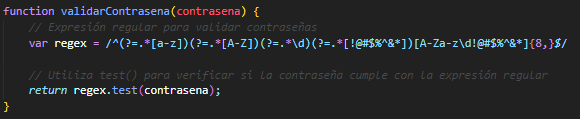
\includegraphics[width=\textwidth]{./img/vulnerabilidades/3.7/2.1.png}
                            \caption{JS de validacion de contraseñas}
                        \end{figure}
                        \item Cambiar las contraseñas de nuestros servicios como phpMyAdmin, MariaDB, etc.
                        \begin{figure}[H]
                            \centering
                            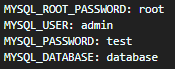
\includegraphics[width=\textwidth]{./img/vulnerabilidades/3.7/2.2.png}
                            \caption{Contraseña antes del cambio}                            
                        \end{figure}
                        \begin{itemize}
                            \item Estas contraseñas se ven dentro del .env el cual no se deberia subir pero al ser un trabajo se ha subido al repositorio.
                        \end{itemize}
                    \end{itemize}
            \clearpage
            \subsection{Invalidacion de sesiones}
                    \subsubsection{Descripción}
                        La invalidación de sesiones se refiere a la práctica de terminar una sesión de usuario cuando el usuario sale de una aplicación o sitio web. Esto puede ayudar a prevenir ataques de tipo secuestro de sesión, en los que un atacante puede tomar el control de una sesión de usuario activa.
                    \subsubsection{Solución}
                        En este punto tambien hemos puesto dos soluciones al problema:
                        \begin{enumerate}
                            \item Hemos añadido un boton de cerrar sesion en la pagina de perfil de usuario.
                            \item La cookie se cierra automaticamente al cerrar el navegador.
                        \end{enumerate}
                        Con estas dos soluciones, si un usuario se olvida de cerrar sesion, el sistema lo hara automaticamente y si un atacante consigue la sesion de un usuario, esta se invalidara de igual forma.
            \clearpage
        \section{Fallos en la integridad de datos y software}
            Los fallos en la integridad de datos y software pueden tener graves consecuencias en la seguridad y confiabilidad de sistemas y aplicaciones. Estos fallos pueden ocurrir debido a diversas razones, y es importante abordarlos adecuadamente para mantener la integridad de los datos y el funcionamiento del software.
            \subsection{Copias de seguridad}
            \clearpage
            \subsection{CI/CD}
                \subsubsection{Descripción}
                    CI/CD es un conjunto de prácticas y herramientas que permiten a los equipos de desarrollo de software entregar cambios de código de forma rápida y fiable. CI/CD es un acrónimo de Integración Continua (CI) y Despliegue Continua (CD). CI/CD es una práctica fundamental para DevOps.
                \subsubsection{Solución}
                    Para solucionar este problema podemos generar un pipeline de CI/CD en GitHub Actions mediante los Workflows.
            \clearpage
        \section{Fallos en la monitorizacion de la seguridad}
            Los fallos en la monitorización de la seguridad se refieren a deficiencias o problemas en los sistemas y procesos diseñados para vigilar y evaluar la seguridad de una red, sistema informático, aplicación o entorno en general.
            \subsection{Auditorias de seguridad}
                \subsubsection{Descripción}
                    Una auditoría de seguridad es un proceso sistemático de evaluación y revisión de sistemas, redes, aplicaciones o entornos tecnológicos con el propósito de identificar vulnerabilidades, debilidades y riesgos de seguridad. El objetivo principal de una auditoría de seguridad es garantizar que los controles de seguridad estén implementados adecuadamente y cumplan con los estándares de seguridad, y proporcionar recomendaciones para mejorar la protección de activos y datos contra amenazas y ataques cibernéticos.
                \subsubsection{Solución}
                    La solucion a este problema es realizar una auditoria de seguridad de forma periodica para detectar posibles fallos de seguridad. 
            \clearpage
            \subsection{Configuracion de logs del sistema}
                \subsubsection{Descripción}
                    Los logs del sistema son una herramienta de seguridad que permite a los administradores de sistemas y a los equipos de seguridad supervisar y analizar la actividad de los sistemas y las redes. Los logs del sistema pueden utilizarse para detectar y analizar incidentes de seguridad, así como para identificar y prevenir posibles amenazas.
                \subsubsection{Solución}
                    Para solucionar este problema, hemos implementado una logica del log del lado del servidor para guardar los logs de los usuarios al cometer errores.
                    \begin{figure}[H]
                        \centering
                        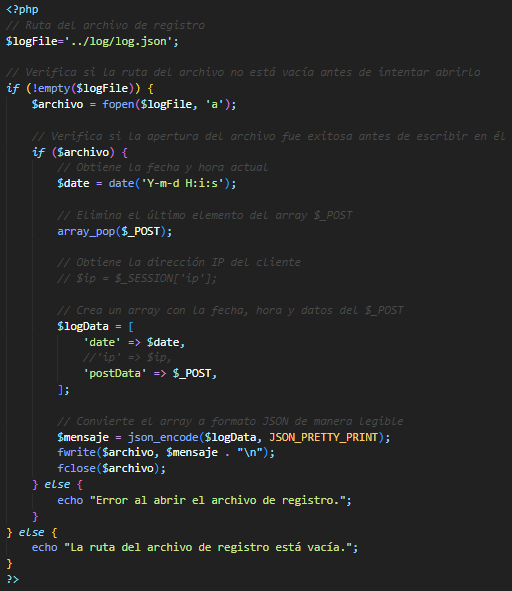
\includegraphics[width=0.9\textwidth]{./img/vulnerabilidades/3.9/2.2.png}
                        \caption{Logs del lado del servidor}
                    \end{figure}
                    
            \clearpage
    \chapter{Segunda auditoria}
        \section{ZAP}
        \clearpage
        \section{sqlmap}
        \clearpage
        \section{nmap}
        \clearpage
        \section{Metaexploit}
        \clearpage
    \chapter{Conclusiones}
    \chapter{Bibliografia}
        \begin{itemize}
            \item OWASP. (2021). Informe de Vulnerabilidades. OWASP. \url{https://owasp.org/www-project-top-ten/}
            \item GPT-3.5. (2023). Respuestas a preguntas varias. OpenAI. \url{https://www.openai.com/}
            \item GitHub Copilot. (2022). Autocompletado. GitHub. \url{https://github.com/features/copilot}
            \item PHP. (2021). Manual de PHP. PHP. \url{https://www.php.net/manual/es/}
            \item reCAPTCHA. (2018). Documentacion de reCAPTCHA. Google. \url{https://developers.google.com/recaptcha/docs/v3}
        \end{itemize}
\end{document}